% ============================================================================
%  RAPPORT DE PROJET — OPTIMISATION CONVEXE
%  Methodes de gradient proximal : ISTA & FISTA
%
%  STRUCTURE MODULAIRE : ce fichier (main.tex) est le chef d'orchestre.
%  Chaque section vit dans son propre fichier sous sections/ et est appelee
%  par \input{}. Chacun travaille sur SON fichier sans toucher aux autres.
%
%  QUI ECRIT QUOI (voir aussi REPARTITION_DETAILLEE.md) :
%    - Membre 1 (moi)   : sections 01, 02, 03  + integration
%    - Membre 2         : section 04 (theorie proximale)        <-- A REMPLIR
%    - Membre 3         : sections 05, 06 (ISTA/FISTA + preuves) <-- A REMPLIR
%    - Membre 4 (Romain): section 07 (etat de l'art)  [DEJA FAIT, a integrer]
%    - Membre 4         : sections 08, 09 (audio + experiences)  <-- A REMPLIR
%    - Membres 1 & 4    : section 10 (conclusion)                <-- A REMPLIR
% ============================================================================
\documentclass[11pt,a4paper]{article}

% --- Encodage & langue ------------------------------------------------------
\usepackage[utf8]{inputenc}
\usepackage[T1]{fontenc}

% --- Maths ------------------------------------------------------------------
\usepackage{amsmath,amssymb,amsthm}
\usepackage{mathtools}
\frenchspacing

% --- Mise en page & figures -------------------------------------------------
\usepackage[margin=2.5cm]{geometry}
\usepackage{graphicx}
\usepackage{booktabs}
\usepackage{array}
\usepackage{caption}
\usepackage{xcolor}
\usepackage{hyperref}
\hypersetup{colorlinks=true, linkcolor=blue!50!black, urlcolor=blue!50!black,
            citecolor=blue!50!black}

% --- Theoremes --------------------------------------------------------------
\theoremstyle{definition}
\newtheorem{definition}{Definition}
\newtheorem{remarque}{Remarque}
\theoremstyle{plain}
\newtheorem{proposition}{Proposition}
\newtheorem{theoreme}{Theoreme}

% --- Macros communes (NOTATIONS PARTAGEES — ne pas diverger) ----------------
\newcommand{\R}{\mathbb{R}}
\newcommand{\norm}[1]{\left\lVert #1 \right\rVert}
\newcommand{\prox}{\operatorname{prox}}
\newcommand{\sign}{\operatorname{sign}}
\newcommand{\argmin}{\operatorname*{arg\,min}}
\newcommand{\softthr}{\operatorname{soft\_threshold}}
\newcommand{\xopt}{x^{\star}}        % solution optimale
\newcommand{\Fopt}{F^{\star}}        % valeur optimale
\newcommand{\T}{^{\top}}             % transposee

% ============================================================================
\begin{document}

% --- Page de garde ----------------------------------------------------------
\begin{titlepage}
\centering
\vspace*{2cm}
{\scshape\large Projet --- Rapport\par}
\vspace{1.5cm}
\rule{\linewidth}{0.4pt}\\[0.4cm]
{\huge\bfseries Methodes de gradient proximal\\[0.3cm]
\large ISTA \& FISTA pour l'optimisation convexe non lisse\par}
\rule{\linewidth}{0.4pt}\\[1.5cm]
{\large Convex optimization \quad 2025--2026\par}
\vspace{2cm}
{\large N'Diaye BALL, Melvyn POMMIER, Romain REN, Jacq VENGADESAN\par}
\vfill
{\large \today\par}
\end{titlepage}

\tableofcontents
\newpage

% ============================================================================
%  PARTIE I — CADRE & PROBLEME  (Membre 1)
% ============================================================================
% ============================================================================
%  SECTION 1 — INTRODUCTION & MOTIVATION        (Membre 1)
% ============================================================================
\section{Introduction et motivation}
\label{sec:intro}

\subsection{Du cours a une question laissee ouverte}

Le cours d'optimisation convexe etablit un resultat fondamental : pour une
fonction convexe sur un ensemble convexe, \emph{tout minimum local est un
minimum global}. Cette propriete --- que nous appellerons la \guillemotleft{}~propriete-or~\guillemotright{}
--- est ce qui rend les problemes convexes \guillemotleft{}~faciles~\guillemotright{} a optimiser : il
n'existe pas de creux sous-optimal dans lequel un algorithme pourrait rester
piege.

Le cours a ensuite presente deux familles de methodes de resolution :
\begin{itemize}
  \item pour un objectif \textbf{lisse} (differentiable), les methodes fondees
        sur le gradient (descente de gradient, methode de Newton) ;
  \item pour un objectif \textbf{lineaire}, l'algorithme du simplexe.
\end{itemize}

Ces deux familles couvrent une large part des problemes, mais elles partagent
une hypothese implicite forte : la descente de gradient et la methode de Newton
exigent que la fonction objectif soit \emph{differentiable}, tandis que le
simplexe ne traite que le cas \emph{lineaire}. Une question reste donc ouverte,
et c'est precisement celle qu'explore ce projet :

\begin{center}
\itshape
Comment resoudre un probleme convexe lorsque la fonction objectif est
convexe mais \textbf{ni lisse, ni lineaire} ?
\end{center}

Ce cas de figure est loin d'etre marginal : il apparait des que l'on ajoute a
un objectif lisse un terme de regularisation non differentiable, situation
omnipresente en traitement du signal, en statistique et en apprentissage
automatique.

\subsection{La technique etudiee : les methodes de gradient proximal}

Pour repondre a cette question, nous etudions une famille de methodes de
premier ordre adaptees au cas non lisse : les \textbf{methodes de gradient
proximal}, et en particulier l'algorithme \textbf{ISTA} (\emph{Iterative
Shrinkage-Thresholding Algorithm}) et son acceleration \textbf{FISTA}
(\emph{Fast ISTA}). Conformement au sujet B, le c\oe ur de ce rapport est
l'\emph{etude de cette technique de resolution} : sa construction, ses garanties
de convergence, et sa comparaison avec les alternatives existantes.

Il importe de souligner d'emblee qu'ISTA et FISTA \emph{ne sont pas des
algorithmes d'apprentissage automatique} : ce sont des algorithmes
d'optimisation convexe, au meme titre que le gradient conjugue ou les methodes
de point interieur cites dans l'enonce du sujet B. Le fait qu'ils soient
frequemment employes en apprentissage ne change rien a leur nature : ils
resolvent un probleme d'optimisation, point.

\subsection{Fil conducteur et application illustrative}

Pour ancrer l'etude dans un probleme concret, nous utilisons comme fil rouge le
probleme du \textbf{LASSO} (regression lineaire avec penalisation $L_1$), qui
est l'instance canonique d'un objectif convexe composite \guillemotleft{}~lisse $+$ non
lisse~\guillemotright{}. En fin de rapport, nous illustrons l'interet pratique de la methode
sur une \textbf{application a la separation de sources audio}
(section~\ref{sec:audio}) ; cette application reste toutefois une
\emph{illustration} et non le sujet : elle rend le probleme tangible et fournit
une evaluation quantitative, mais l'analyse demeure centree sur l'optimisation.

\subsection{Organisation du rapport}

Le rapport s'organise en trois temps. La premiere partie pose le cadre :
rappels du cours mobilises (section~\ref{sec:rappels}) puis formulation precise
du probleme composite et preuve de sa convexite (section~\ref{sec:probleme}).
La deuxieme partie constitue le c\oe ur theorique : les outils de l'optimisation
non lisse, dont l'operateur proximal (section~\ref{sec:theorie}), puis les
algorithmes ISTA (section~\ref{sec:ista}) et FISTA (section~\ref{sec:fista})
avec leurs preuves de convergence. La troisieme partie met la methode en
perspective : etat de l'art comparatif (section~\ref{sec:etatart}), application
audio (section~\ref{sec:audio}) et experiences numeriques
(section~\ref{sec:exp}). La section~\ref{sec:conclusion} conclut.

% ============================================================================
%  SECTION 2 — RAPPELS ET CADRE THEORIQUE        (Membre 1)
% ============================================================================
\section{Rappels et cadre theorique}
\label{sec:rappels}

Cette section rassemble les notions du cours mobilisees dans la suite. Elle ne
vise pas l'exhaustivite mais fixe le vocabulaire, les notations et les
proprietes sur lesquelles reposent les sections suivantes.

\subsection{Probleme d'optimisation}

Un probleme d'optimisation consiste a minimiser (ou maximiser) une fonction
objectif $f : A \to \R$ sur un ensemble admissible $A$ :
\[
  \min_{x \in A} \; f(x).
\]
Un element $x \in A$ est une \emph{solution admissible} ; une solution qui
realise le minimum est une \emph{solution optimale}, notee $\xopt$. Lorsque
l'ensemble admissible est decrit par des contraintes d'inegalite, on ecrit
\[
  \min_{x \in \R^{n}} f(x)
  \quad\text{sous contraintes}\quad
  c_i(x) \le b_i, \quad i = 1, \dots, m.
\]

\subsection{Convexite}

\begin{definition}[Ensemble convexe]
Un ensemble $A \subseteq \R^{n}$ est \emph{convexe} si, pour tout couple de
points de $A$, le segment qui les joint est entierement contenu dans $A$ :
\[
  \forall x, y \in A,\ \forall \lambda \in [0,1] :\quad
  \lambda x + (1-\lambda) y \in A.
\]
\end{definition}

\begin{definition}[Fonction convexe]
Une fonction $f : \R^{n} \to \R$ est \emph{convexe} si
\[
  \forall x, y \in \R^{n},\ \forall \lambda \in [0,1] :\quad
  f\big(\lambda x + (1-\lambda) y\big)
  \le \lambda f(x) + (1-\lambda) f(y).
\]
Geometriquement, tout segment reliant deux points du graphe se situe au-dessus
(ou sur) le graphe. Lorsque l'inegalite est \emph{stricte} pour $x \neq y$ et
$\lambda \in {]0,1[}$, la fonction est dite \emph{strictement convexe}.
\end{definition}

Deux proprietes de stabilite, etablies en travaux diriges, seront utilisees
pour montrer que notre probleme est convexe :
\begin{proposition}[Stabilite de la convexite]
\label{prop:stabilite}
\leavevmode
\begin{enumerate}
  \item Un demi-espace $\{x \in \R^{n} : a\T x \le b\}$ est un ensemble convexe ;
        une intersection d'ensembles convexes est convexe.
  \item Une somme de fonctions convexes est convexe ; le produit d'une fonction
        convexe par un scalaire positif est convexe.
\end{enumerate}
\end{proposition}

\subsection{La propriete fondamentale, et ses limites}

\begin{theoreme}[Propriete-or]
\label{th:or}
Tout minimum local d'une fonction convexe est un minimum global.
\end{theoreme}

C'est cette propriete qui justifie l'interet des problemes convexes : un
algorithme qui converge vers un minimum local converge en realite vers
l'optimum global. Une precision s'impose toutefois, car elle conditionne la
lecture de nos resultats experimentaux.

\begin{remarque}[Convexite et unicite]
\label{rem:unicite}
La convexite garantit l'unicite de la \emph{valeur optimale} $\Fopt$, mais
\textbf{pas} celle du \emph{minimiseur} $\xopt$. L'ensemble des minimiseurs
peut etre reduit a un point, mais aussi former tout un segment --- le cours en
donne d'ailleurs un exemple en programmation lineaire, ou l'ensemble des
solutions optimales est un segment entier. L'unicite du minimiseur requiert une
hypothese plus forte, la \emph{stricte} convexite. Comme nous le verrons
(section~\ref{sec:probleme}), le LASSO n'est pas strictement convexe en general ;
on ne pourra donc affirmer que la convergence se fait vers une \emph{meme valeur}
$\Fopt$, et non necessairement vers un \emph{meme point} $\xopt$.
\end{remarque}

\subsection{Programmation lineaire et quadratique}

Le cours a etudie en detail la \emph{programmation lineaire}, cas particulier ou
objectif et contraintes sont lineaires, resolue par l'algorithme du simplexe.
Notre probleme generalise ce cadre dans une direction differente : l'objectif y
sera \emph{quadratique} (donc convexe mais non lineaire) et augmente d'un terme
de regularisation \emph{non differentiable}. Ni le simplexe ni la descente de
gradient classique ne s'y appliquent directement, ce qui motive l'introduction
des outils de la section~\ref{sec:theorie}.

% ============================================================================
%  SECTION 3 — LE PROBLEME : MINIMISATION CONVEXE COMPOSITE   (Membre 1)
% ============================================================================
\section{Le probleme : minimisation convexe composite}
\label{sec:probleme}

\subsection{Un probleme inverse sous-determine}

Placons-nous dans une situation typique du traitement du signal. On observe un
vecteur de mesures $y \in \R^{n}$, relie a un signal inconnu $x \in \R^{p}$ par
une matrice connue $A \in \R^{n \times p}$ :
\[
  y = A x + \varepsilon,
\]
ou $\varepsilon$ represente un bruit. Le point determinant est que l'on dispose
de \emph{moins de mesures que d'inconnues} ($p > n$) : le systeme est
\emph{sous-determine} et admet une infinite de solutions compatibles avec $y$.
Sans information supplementaire, le probleme est mal pose.

L'information que l'on ajoute est une hypothese de \textbf{parcimonie}
(\emph{sparsity}) : le vrai signal $x$ ne possede que peu de composantes non
nulles. Cette hypothese est realiste --- de nombreux signaux naturels admettent
une representation creuse dans une base adaptee --- et suffit a rendre le
probleme bien pose.

\subsection{Formulation : le LASSO}

Pour retrouver $x$, on minimise un objectif en deux termes, l'un mesurant la
fidelite aux donnees, l'autre favorisant la parcimonie :
\begin{equation}
\label{eq:lasso}
  \boxed{\;
  \min_{x \in \R^{p}} \; F(x)
  = \underbrace{\tfrac{1}{2}\,\norm{A x - y}_2^{2}}_{f(x)\ \text{(lisse)}}
  \;+\; \lambda \underbrace{\norm{x}_1}_{g(x)\ \text{(non lisse)}}
  \;}
\end{equation}
ou $\norm{x}_1 = \sum_{i=1}^{p} |x_i|$ et $\lambda > 0$ regle le compromis entre
les deux termes. Ce probleme est connu sous le nom de \textbf{LASSO}
(\emph{Least Absolute Shrinkage and Selection Operator}). On notera dans toute
la suite
\[
  f(x) = \tfrac{1}{2}\norm{A x - y}_2^{2},
  \qquad
  g(x) = \lambda \norm{x}_1,
  \qquad
  F = f + g .
\]
Le terme $f$ est differentiable, de gradient
\begin{equation}
\label{eq:gradf}
  \nabla f(x) = A\T (A x - y),
\end{equation}
qui est \emph{lipschitzien} de constante $L = \norm{A\T A}_2$ (la plus grande
valeur propre de $A\T A$). Cette constante jouera un role central dans le choix
du pas des algorithmes (sections~\ref{sec:ista} et~\ref{sec:fista}).

\subsection{Le probleme est convexe}

Verifions que~\eqref{eq:lasso} entre bien dans le cadre du cours.

\begin{proposition}
\label{prop:convexe}
La fonction objectif $F = f + g$ est convexe sur $\R^{p}$, et l'ensemble
admissible $\R^{p}$ est convexe. Le probleme~\eqref{eq:lasso} est donc un
probleme d'optimisation convexe.
\end{proposition}

\begin{proof}
On procede terme a terme.
\begin{enumerate}
  \item \emph{$f$ est convexe.} La fonction $f(x) = \tfrac12\norm{Ax-y}_2^2$ est
        quadratique, de matrice hessienne $\nabla^2 f(x) = A\T A$. Pour tout
        $u \in \R^{p}$, $u\T A\T A\, u = \norm{A u}_2^2 \ge 0$, donc $A\T A$ est
        semi-definie positive : $f$ est convexe.
  \item \emph{$g$ est convexe.} La norme $\norm{\cdot}_1$ est une norme, donc
        convexe (inegalite triangulaire et homogeneite) ; multipliee par
        $\lambda > 0$, elle reste convexe
        (proposition~\ref{prop:stabilite}).
  \item \emph{$F$ est convexe.} Comme somme de deux fonctions convexes, $F$ est
        convexe (proposition~\ref{prop:stabilite}).
  \item \emph{L'ensemble admissible.} Il s'agit de $\R^{p}$ tout entier, qui est
        trivialement convexe.
\end{enumerate}
La propriete-or (theoreme~\ref{th:or}) s'applique donc : tout minimum local
de~\eqref{eq:lasso} est global.
\end{proof}

\begin{remarque}[Pas de stricte convexite en general]
\label{rem:pas-stricte}
Conformement a la remarque~\ref{rem:unicite}, $F$ n'est pas strictement convexe
des que $p > n$. En effet, $f$ n'est strictement convexe que si $A\T A$ est
\emph{definie} positive, c'est-a-dire si $A$ est injective ; or, avec plus de
colonnes que de lignes ($p > n$), $A$ possede un noyau non trivial. Quant a
$g = \lambda\norm{\cdot}_1$, elle est convexe mais pas strictement. On ne peut
donc pas garantir l'unicite du minimiseur $\xopt$ : les algorithmes des sections
suivantes convergeront vers une \emph{meme valeur optimale} $\Fopt$, sans que le
point atteint soit necessairement unique.
\end{remarque}

\subsection{Pourquoi les methodes du cours echouent}
\label{subsec:echec}

Le terme $g(x) = \lambda\norm{x}_1$ fait intervenir des valeurs absolues
$|x_i|$. Or la fonction $t \mapsto |t|$ presente un \emph{point anguleux} en
$0$ : sa derivee vaut $-1$ a gauche et $+1$ a droite, et \textbf{n'existe pas en
$0$}. Cette simple observation a des consequences directes :
\begin{itemize}
  \item la \textbf{descente de gradient} requiert $\nabla F$, qui n'est pas
        defini la ou des composantes de $x$ s'annulent --- c'est-a-dire
        precisement la ou se trouve la solution recherchee, puisqu'elle est
        creuse ;
  \item la \textbf{methode de Newton} exige en outre la hessienne de $F$, encore
        moins disponible ;
  \item le \textbf{simplexe} ne traite que les objectifs lineaires, alors que le
        notre est quadratique.
\end{itemize}
Il nous faut donc un outil capable de gerer ce point anguleux sans recourir a la
differentiabilite. Cet outil est l'\emph{operateur proximal}, introduit a la
section suivante.


% ============================================================================
%  PARTIE II — THEORIE & ALGORITHMES  (Membres 2 et 3)
% ============================================================================
% ============================================================================
%  SECTION 4 — OUTILS THEORIQUES : SOUS-DIFFERENTIEL & OPERATEUR PROXIMAL
%  >>> A REMPLIR PAR LE MEMBRE 2 <<<
%
%  Objectif de la section : fournir la fondation theorique dont dependent les
%  preuves des sections 5 (ISTA) et 6 (FISTA). C'est le PIVOT du rapport.
%
%  Contenu attendu (voir REPARTITION_DETAILLEE.md) :
%    - Sous-differentiel d'une fonction convexe non lisse ; cas de |t| en 0
%      (l'ensemble des pentes [-1, 1]).
%    - Condition d'optimalite : 0 \in \partial F(x*).
%    - Definition de l'operateur proximal :
%        prox_{t g}(z) = argmin_u  g(u) + (1/2t) ||u - z||^2
%      + interpretation geometrique.
%    - DERIVATION COMPLETE du seuillage doux (prox de lambda||.||_1) :
%      separation coordonnee par coordonnee -> sign(z)*max(|z|-t*lambda, 0).
%    - Propriete de non-expansivite du prox (utile pour les preuves de conv.).
%
%  Notations a respecter (definies dans main.tex) :
%    \prox, \softthr, \norm{.}, \argmin, \sign, \xopt, \Fopt, \R, \T
%  Reutiliser : F = f + g, f(x)=1/2||Ax-y||^2, g(x)=lambda||x||_1, L=||A^T A||.
% ============================================================================
\section{Outils theoriques : sous-differentiel et operateur proximal}
\label{sec:theorie}

% --- [MEMBRE 2] Ecrire la section ici. Squelette suggere ci-dessous. --------

\subsection{Le sous-differentiel}
% TODO (Membre 2)

\subsection{Condition d'optimalite}
% TODO (Membre 2)

\subsection{L'operateur proximal}
% TODO (Membre 2)

\subsection{Derivation du seuillage doux}
% TODO (Membre 2) : c'est le coeur. La formule a etablir est
% \prox_{t\lambda\norm{\cdot}_1}(z)_i = \sign(z_i)\max(|z_i| - t\lambda, 0).

\subsection{Non-expansivite}
% TODO (Membre 2)
   % Membre 2  <-- A REMPLIR
% ============================================================================
%  SECTION 5 — ISTA : ITERATIVE SHRINKAGE-THRESHOLDING
%  >>> A REMPLIR PAR LE MEMBRE 3 <<<
%
%  Depend de la section 4 (operateur proximal) du Membre 2.
%
%  Contenu attendu (voir REPARTITION_DETAILLEE.md) :
%    - Construction d'ISTA comme MAJORATION-MINIMISATION : a chaque pas, on
%      minimise un majorant quadratique de f + le terme g ; montrer que cela
%      redonne exactement "pas de gradient + prox".
%    - Iteration :
%        x_{k+1} = \softthr( x_k - t \nabla f(x_k), t\lambda )
%      avec \nabla f(x) = A^T(Ax - y) et pas t <= 1/L, L = ||A^T A||.
%    - PREUVE DE CONVERGENCE EN O(1/k) (argument du gradient Lipschitz).
%
%  Penser a renvoyer a la figure de convergence de la section 9 (experiences).
% ============================================================================
\section{ISTA : l'algorithme de gradient proximal}
\label{sec:ista}

% --- [MEMBRE 3] Ecrire la section ici. Squelette suggere ci-dessous. --------

\subsection{Idee : separer la partie lisse et la partie non lisse}
% TODO (Membre 3)

\subsection{Construction par majoration-minimisation}
% TODO (Membre 3)

\subsection{L'algorithme}
% TODO (Membre 3) : pseudo-code + role du pas t <= 1/L.

\subsection{Convergence en $O(1/k)$}
% TODO (Membre 3) : enonce + preuve.
                 % Membre 3  <-- A REMPLIR
% ============================================================================
%  SECTION 6 — FISTA : FAST ISTA
%  >>> A REMPLIR PAR LE MEMBRE 3 <<<
%
%  Depend des sections 4 (prox) et 5 (ISTA).
%
%  Contenu attendu (voir REPARTITION_DETAILLEE.md) :
%    - Le momentum de Nesterov : d'ou vient le point extrapole y_k.
%    - Iteration :
%        x_k     = \softthr( y_k - t \nabla f(y_k), t\lambda )
%        t_{k+1} = (1 + sqrt(1 + 4 t_k^2)) / 2
%        y_{k+1} = x_k + ((t_k - 1)/t_{k+1}) (x_k - x_{k-1})
%    - PREUVE (ou esquisse detaillee) DE LA CONVERGENCE EN O(1/k^2)
%      (suite d'energie de Beck & Teboulle, 2009).
%    - Discussion des OSCILLATIONS / non-monotonie ; variantes "restart".
%
%  Renvoyer a la figure de convergence (section 9) qui montre O(1/k) vs O(1/k^2).
% ============================================================================
\section{FISTA : acceleration par momentum}
\label{sec:fista}

% --- [MEMBRE 3] Ecrire la section ici. Squelette suggere ci-dessous. --------

\subsection{Du gradient proximal au momentum de Nesterov}
% TODO (Membre 3)

\subsection{L'algorithme}
% TODO (Membre 3) : pseudo-code, une ligne de plus qu'ISTA.

\subsection{Convergence en $O(1/k^2)$}
% TODO (Membre 3) : enonce + preuve/esquisse.

\subsection{Non-monotonie et variantes a restart}
% TODO (Membre 3) : commenter les oscillations observees experimentalement.
                % Membre 3  <-- A REMPLIR

% ============================================================================
%  PARTIE III — MISE EN PERSPECTIVE & EXPERIENCES  (Membre 4)
% ============================================================================
% ============================================================================
%  SECTION 7 — ETAT DE L'ART : SITUER ISTA ET FISTA       (Membre 4 — Romain)
%
%  NOTE D'INTEGRATION (Membre 1) : ce contenu reprend l'etat de l'art redige par
%  Romain. Il a ete renumerote (section 7, anciennement "0") et aligne sur les
%  macros communes (\prox, \softthr, \norm, \T, \Fopt...). Le fond et la
%  structure d'origine (4 familles + synthese + discussion) sont conserves.
% ============================================================================
\section{Etat de l'art : situer ISTA et FISTA}
\label{sec:etatart}

ISTA et FISTA ne sont qu'un point dans un paysage plus large de methodes
capables de resoudre le probleme composite~\eqref{eq:lasso}. Le critere
d'evaluation du sujet B demande explicitement de comparer les alternatives :
c'est l'objet de cette section. On retient quatre familles --- les methodes de
gradient proximal, la descente par coordonnees, l'ADMM et le Newton proximal ---
et on confronte chacune a ISTA/FISTA selon trois axes juges decisifs en
pratique : la vitesse de convergence (en nombre d'iterations), le cout d'une
iteration, et la structure de probleme pour laquelle la methode est la mieux
adaptee.

\subsection{Le cadre commun : minimiser une somme $f + g$}

Toutes ces methodes attaquent le meme objet : une somme d'une partie lisse $f$
(de gradient $L$-lipschitzien, $L = \norm{A\T A}_2$) et d'une partie convexe non
lisse $g$. Ce qui les distingue, c'est la maniere dont elles exploitent cette
structure :
\begin{itemize}
  \item \textbf{ISTA/FISTA} separent $f$ et $g$ : un pas de gradient sur $f$,
        puis l'operateur proximal de $g$ (le seuillage doux). C'est l'approche
        \emph{full-gradient} : chaque iteration met a jour tout le vecteur $x$.
  \item La \textbf{descente par coordonnees} exploite la separabilite de
        $g = \lambda\norm{\cdot}_1 = \sum_j \lambda |x_j|$ pour ne mettre a jour
        qu'une coordonnee a la fois.
  \item L'\textbf{ADMM} dedouble les variables (une copie pour $f$, une pour $g$)
        et les recoud via un multiplicateur.
  \item Le \textbf{Newton proximal} exploite en plus la courbure de $f$ (la
        hessienne $A\T A$), la ou ISTA/FISTA n'utilisent que le gradient.
\end{itemize}
On reconnait ISTA/FISTA comme le membre le plus \guillemotleft{}~elementaire~\guillemotright{} de cette
famille : ordre 1, separation minimale, aucune structure supplementaire
exploitee. Cette sobriete est a la fois leur force (generalite, simplicite, cout
par iteration faible) et leur limite (convergence sous-lineaire).

\subsection{Descente par coordonnees}

\paragraph{Principe.} Plutot que de bouger toutes les composantes de $x$
ensemble, on les met a jour une par une : on fixe toutes les coordonnees sauf la
$j$-ieme et on minimise $F$ exactement selon $x_j$. Pour le LASSO, ce
sous-probleme a une variable admet une solution explicite --- un seuillage doux
sur le residu partiel :
\[
  x_j \leftarrow \softthr\!\left(
    \frac{1}{\norm{a_j}_2^{2}}\, a_j\T\big(y - A x + a_j x_j\big),\;
    \frac{\lambda}{\norm{a_j}_2^{2}}
  \right),
\]
ou $a_j$ est la $j$-ieme colonne de $A$. On balaie les coordonnees cycliquement
(ou aleatoirement) jusqu'a stabilisation.

\paragraph{Vitesse.} Pour le LASSO, la descente par coordonnees converge a un
taux asymptotiquement \emph{lineaire}, $F(x_k) - \Fopt = O(\rho^{k})$ avec
$\rho < 1$, une fois identifie le support de la solution --- bien mieux que le
$O(1/k)$ d'ISTA et le $O(1/k^2)$ de FISTA dans ce regime final. C'est d'ailleurs
la methode au c\oe ur de \texttt{glmnet}, l'implementation de reference du LASSO
en statistique.

\paragraph{Cout par iteration.} Une mise a jour de coordonnee est tres bon
marche ($O(n)$ si l'on maintient le residu $r = y - Ax$ de maniere
incrementale). Un balayage complet des $p$ coordonnees coute $O(np)$, comparable
a une iteration d'ISTA. L'avantage decisif est l'identification automatique du
support : les coordonnees nulles le restent.

\paragraph{Quand la preferer.} Lorsque la penalite est separable (comme
$\norm{\cdot}_1$) et que les colonnes de $A$ sont peu correlees ; choix par
defaut en grande dimension statistique ($p \gg n$) avec solution tres
parcimonieuse. En revanche, la methode est intrinsequement sequentielle (donc
difficile a paralleliser) et perd son avantage quand $g$ n'est pas separable.

\subsection{ADMM (Alternating Direction Method of Multipliers)}

\paragraph{Principe.} On reformule le probleme en dedoublant la variable via une
copie $z$ et la contrainte $x = z$ :
\[
  \min_{x, z}\; f(x) + g(z) \quad\text{s.c.}\quad x = z,
\]
puis on minimise le lagrangien augmente
$\mathcal{L}_\rho(x,z,u) = f(x) + g(z) + \tfrac{\rho}{2}\norm{x - z + u}_2^2$ en
alternant trois pas :
\[
\begin{aligned}
  x_{k+1} &\leftarrow \argmin_x\; f(x) + \tfrac{\rho}{2}\norm{x - z_k + u_k}_2^2
            && \text{(systeme lineaire),}\\
  z_{k+1} &\leftarrow \prox_{g/\rho}(x_{k+1} + u_k)
            && \text{(seuillage doux),}\\
  u_{k+1} &\leftarrow u_k + x_{k+1} - z_{k+1}
            && \text{(montee de gradient duale).}
\end{aligned}
\]
Le pas en $z$ est exactement le seuillage doux deja implemente pour ISTA.

\paragraph{Vitesse.} En pratique, l'ADMM atteint une precision moderee en
nettement moins d'iterations qu'ISTA (souvent quelques dizaines). Theoriquement,
sa vitesse est $O(1/k)$ pour des objectifs convexes generaux, et lineaire sous
hypotheses fortes ; elle depend toutefois sensiblement du parametre de penalite
$\rho$, dont le reglage est delicat.

\paragraph{Cout par iteration.} C'est le point faible : le pas en $x$ exige de
resoudre un systeme lineaire $(A\T A + \rho I)\,x = b$. Si $A$ est fixe, on
factorise $A\T A + \rho I$ une seule fois (Cholesky, $O(p^3)$) et chaque
iteration ne coute plus que deux substitutions $O(p^2)$ : l'ADMM devient alors
tres competitif. Mais si $\rho$ change ou si $A$ est trop grande pour etre
factorisee, ce pas redevient couteux. Autre nuance : contrairement a ISTA/FISTA
et a la descente par coordonnees, les iteres d'ADMM ne sont pas exactement
parcimonieux avant convergence (seul le bloc $z$ l'est).

\paragraph{Quand le preferer.} Quand le probleme se decompose naturellement
(regularisations multiples, contraintes, problemes distribues), ou quand la
factorisation peut etre amortie sur de nombreuses iterations. L'ADMM brille par
sa modularite : on peut remplacer $g$ par n'importe quelle fonction dont on sait
calculer le prox.

\subsection{Newton proximal}

\paragraph{Principe.} ISTA majore $f$ par un modele quadratique isotrope
$\tfrac{1}{2t}\norm{x - x_k}_2^2$ (une \guillemotleft{}~boule~\guillemotright{}). Le Newton proximal
remplace ce modele par la vraie courbure : il utilise la hessienne
$H = \nabla^2 f = A\T A$ et resout, a chaque pas, un sous-probleme de la forme
\[
  x_{k+1} = \argmin_x\;
    \nabla f(x_k)\T (x - x_k)
    + \tfrac{1}{2}(x - x_k)\T H (x - x_k)
    + g(x),
\]
soit un LASSO local, resolu approximativement par un solveur interne (souvent de
la descente par coordonnees). On peut aussi le voir comme une methode de Newton
semi-lisse appliquee a la condition d'optimalite $0 \in \partial F(\xopt)$.

\paragraph{Vitesse.} C'est le regime le plus rapide pres de l'optimum :
convergence superlineaire, voire quadratique localement
($\norm{x_{k+1} - \xopt} = O(\norm{x_k - \xopt}^2)$). La ou FISTA demande des
centaines d'iterations pour gagner les derniers chiffres de precision, le Newton
proximal les obtient en une poignee de pas.

\paragraph{Cout par iteration.} Tres eleve : chaque iteration exige une
information de second ordre (la hessienne ou son action) et la resolution d'un
sous-probleme interne. Le pari n'est gagnant que si le faible nombre
d'iterations externes compense leur cout unitaire --- ce qui suppose en general
une phase d'amorcage par une methode d'ordre 1 (typiquement FISTA) avant de
basculer sur Newton.

\paragraph{Quand le preferer.} Quand on vise une haute precision sur un probleme
de taille moderee, ou quand $f$ est bien conditionnee et la hessienne
exploitable. A l'inverse, en tres grande dimension ou former $A\T A$ est
prohibitif, les methodes d'ordre 1 restent incontournables.

\subsection{Synthese comparative}

Le tableau~\ref{tab:comparatif} recapitule les compromis. Aucune methode ne
domine partout : le bon choix depend de la precision visee, de la taille du
probleme et de la structure exploitable.

\begin{table}[h]
\centering
\small
\begin{tabular}{@{}lllll@{}}
\toprule
\textbf{Methode} & \textbf{Ordre} & \textbf{Vitesse} &
\textbf{Cout / iteration} & \textbf{Terrain de predilection} \\
\midrule
ISTA            & 1 & $O(1/k)$            & faible ($Ax$, $A\T r$)        & socle simple, general \\
FISTA           & 1 & $O(1/k^2)$          & faible (idem ISTA)            & precision moyenne, par defaut \\
Coord. descent  & 1 & lineaire (asympt.)  & tres faible (1 coord.)        & $g$ separable, $p \gg n$ \\
ADMM            & 1 & $O(1/k)$, $\rho$-dep.& moyen (systeme lin.)         & decomposable, distribue \\
Prox. Newton    & 2 & superlin. / quadr.  & eleve (hessienne + interne)   & haute precision, taille moderee \\
\bottomrule
\end{tabular}
\caption{Comparaison des principales methodes pour le LASSO. \guillemotleft{}~Ordre~\guillemotright{}
designe l'ordre de l'information derivee utilisee. Le regime lineaire de la
descente par coordonnees et le regime quadratique de Newton sont \emph{locaux}
(atteints pres de l'optimum).}
\label{tab:comparatif}
\end{table}

\paragraph{Discussion des compromis.} Trois arbitrages structurent ce paysage.
\begin{itemize}
  \item \emph{Vitesse vs. cout par iteration.} Plus une methode converge en peu
        d'iterations (Newton, ADMM), plus ces iterations sont cheres. ISTA/FISTA
        font le pari inverse : des iterations tres bon marche, quitte a en faire
        beaucoup. En grande dimension, ce pari est souvent le bon.
  \item \emph{Generalite vs. exploitation de structure.} ISTA/FISTA ne demandent
        que $\nabla f$ et le prox de $g$ --- d'ou leur generalite. La descente
        par coordonnees exige la separabilite de $g$ ; le Newton proximal une
        courbure exploitable ; l'ADMM une decomposition commode. Ces hypotheses,
        quand elles tiennent, paient.
  \item \emph{Memoire et robustesse.} ISTA/FISTA et la descente par coordonnees
        ont une empreinte memoire minimale. L'ADMM stocke une variable duale et
        idealement une factorisation ; le Newton proximal manipule de
        l'information de second ordre, le plus gourmand. Cote robustesse, ISTA
        est le plus previsible ; FISTA introduit des oscillations non monotones
        (cf.~section~\ref{sec:exp}) que des variantes \emph{restart} corrigent ;
        l'ADMM est sensible a $\rho$ ; Newton depend d'un bon amorcage.
\end{itemize}

\paragraph{Position d'ISTA/FISTA.} En definitive, FISTA occupe un point
d'equilibre remarquable : sans hypothese de structure au-dela de la separation
$f + g$, sans parametre delicat a regler, avec un cout par iteration minimal, il
atteint le meilleur taux possible pour une methode du premier ordre
($O(1/k^2)$, optimal au sens de Nesterov). C'est ce qui en fait le \guillemotleft{}~cheval de
bataille~\guillemotright{} par defaut, et la brique de base a partir de laquelle les autres
methodes se construisent ou se comparent --- d'ou sa place centrale dans ce
projet, les autres approches servant de points de repere pour en mesurer les
forces et les limites.
        % Membre 4  [contenu de Romain]
% ============================================================================
%  SECTION 8 — APPLICATION : SEPARATION DE SOURCES AUDIO
%  >>> A REMPLIR PAR LE MEMBRE 4 <<<  (application BONUS, pas le coeur du sujet)
%
%  Contenu attendu (voir REPARTITION_DETAILLEE.md) :
%    - Pipeline : signal -> representation temps-frequence (STFT) -> LASSO
%      resolu par FISTA -> reconstruction.
%    - Montrer que la separation se ramene au probleme (eq:lasso).
%    - Metrique SDR (Signal-to-Distortion Ratio), ecoute avant/apres.
%    - Necessite librosa (dependance optionnelle).
% ============================================================================
\section{Application : separation de sources audio}
\label{sec:audio}

% --- [MEMBRE 4] Ecrire la section ici. ---
% TODO : rappeler que c'est une illustration, le coeur restant ISTA/FISTA.
   % Membre 4  <-- A REMPLIR
% ============================================================================
%  SECTION 9 — EXPERIENCES NUMERIQUES
%  >>> A REMPLIR PAR LE MEMBRE 4 <<<
%
%  Contenu attendu (voir REPARTITION_DETAILLEE.md) :
%    - Validation sur signal synthetique (cf. notebook) : qualite de
%      recuperation vs nombre de vrais coefficients.
%    - COURBE DE CONVERGENCE ISTA vs FISTA (la figure-phare) : illustre
%      empiriquement O(1/k) vs O(1/k^2). Inserer la figure exportee depuis
%      /experiments (style graphique commun du notebook).
%    - Etude de sensibilite : effet de lambda (parcimonie vs fidelite) et du
%      pas t sur la convergence.
%    - Commenter les oscillations de FISTA (lien avec section 6).
%
%  Pour inserer la figure :
%    \begin{figure}[h]\centering
%      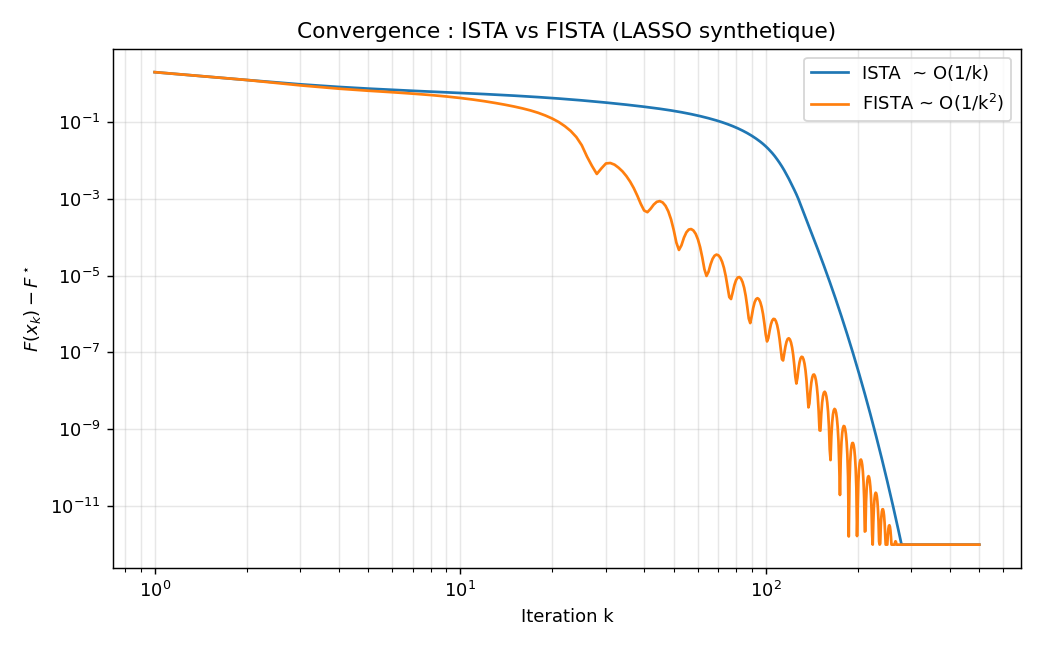
\includegraphics[width=.7\linewidth]{figures/convergence_ista_fista.png}
%      \caption{...}\label{fig:conv}
%    \end{figure}
% ============================================================================
\section{Experiences numeriques}
\label{sec:exp}

% --- [MEMBRE 4] Ecrire la section ici. ---
% TODO
         % Membre 4  <-- A REMPLIR

% ============================================================================
%  CONCLUSION  (Membres 1 & 4)
% ============================================================================
% ============================================================================
%  SECTION 10 — CONCLUSION
%  >>> A REMPLIR PAR LES MEMBRES 1 & 4 <<<
%
%  Contenu attendu :
%    - Bilan : on a etudie une technique de resolution de programmes convexes
%      non lisses (gradient proximal), prouve ses garanties (O(1/k), O(1/k^2)),
%      compare aux alternatives (section 7), illustre sur l'audio (section 8).
%    - Rappeler le positionnement : FISTA = coeur, audio = application.
%    - Ouvertures : FISTA a restart, pas adaptatif (backtracking), extension
%      aux problemes non convexes.
% ============================================================================
\section{Conclusion}
\label{sec:conclusion}

% --- [MEMBRES 1 & 4] Ecrire la conclusion ici. ---
% TODO
          % <-- A REMPLIR

\end{document}
